% This must be in the first 5 lines to tell arXiv to use pdfLaTeX, which is strongly recommended.
\pdfoutput=1
% In particular, the hyperref package requires pdfLaTeX in order to break URLs across lines.

\documentclass[11pt]{article}

% Remove the "review" option to generate the final version.
\usepackage[review]{ACL2023}

% Standard package includes
\usepackage{times}
\usepackage{latexsym}

% For proper rendering and hyphenation of words containing Latin characters (including in bib files)
\usepackage[T1]{fontenc}
% For Vietnamese characters
% \usepackage[T5]{fontenc}
% See https://www.latex-project.org/help/documentation/encguide.pdf for other character sets

% This assumes your files are encoded as UTF8
\usepackage[utf8]{inputenc}

% This is not strictly necessary, and may be commented out.
% However, it will improve the layout of the manuscript,
% and will typically save some space.
\usepackage{microtype}

% This is also not strictly necessary, and may be commented out.
% However, it will improve the aesthetics of text in
% the typewriter font.
\usepackage{inconsolata}
\usepackage{graphicx}

% If the title and author information does not fit in the area allocated, uncomment the following
%
%\setlength\titlebox{<dim>}
%
% and set <dim> to something 5cm or larger.

\title{Instructions for ACL 2023 Proceedings}



\author{Leixin Zhang \\ 
    Computational Linguistics\\
    Seminar für Sprachwissenschaft,
    Universität Tübingen, Germany \\ 
    \texttt{leixin.zhang@student.uni-tuebingen.de}
    }%\\\And
  % Second Author \\
  % Affiliation / Address line 1 \\
  % Affiliation / Address line 2 \\
  % Affiliation / Address line 3 \\
  % \texttt{email@domain} \\}

\begin{document}
\maketitle
\begin{abstract}
This is abstract
\end{abstract}

\section{Introduction}


\section{Previous studies}

\section{Methodology}


\section{Evaluating Sentence Embeddings with Gaussian Mixture}

This section presents an unsupervised approach for evaluating the separability of sentence embeddings. We measure label separability pairwisely using a Gaussian Mixture model and calculate the F-score of the unsupervised clustered labels with the true labels.

The Gaussian Mixture model is a probabilistic model that assumes that each cluster follows a Gaussian (or normal) distribution and estimates the weight of the density function for each cluster \cite{reynolds2009gaussian,5298967}. We assume that the sentence vectors of two distinct classes should achieve high accuracy with Gaussian Mixture if they are displayed in a Gaussian distribution in space and are separable from each other.

However, there is a potential limitation to using this method. The separability and accuracy score may be underestimated if two clusters are not normally distributed, as illustrated in Figure \ref{fig:cirle}.


\begin{figure}[htp]
    \centering
    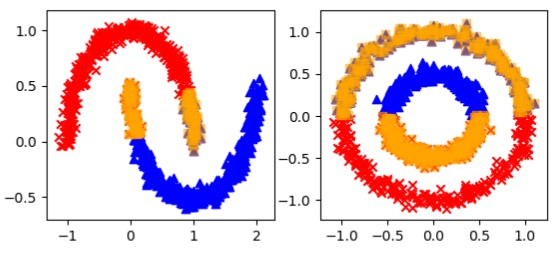
\includegraphics[scale=0.4]{Circle.jpg}
    \caption{Cases that Gaussian Mixture Underestimate the Separability of Two Clusters}
    \label{fig:cirle}
\end{figure}


Our evaluation results show that out of 78 pairs of derivation classes, 7 pairs achieved an accuracy score above 90\%, 24 pairs above 80\%, and 47 pairs above 60\%, as depicted in Figure \ref{fig:GM}.

In particular, the class `ban' demonstrates good separability with many other classes, achieving an accuracy score of 0.982 with `past', 0.980 with `formal sentence', 0.942 with `minimal change', and 0.937 with `future', among other pairs.

Additionally, our evaluation results reveal that tenses are generally well-separated, with an accuracy score of 0.90 for `past' and future' classes, and an accuracy score of 0.924 for `simple sentence' and `future' classes.

\begin{figure}[htp]
    \centering
    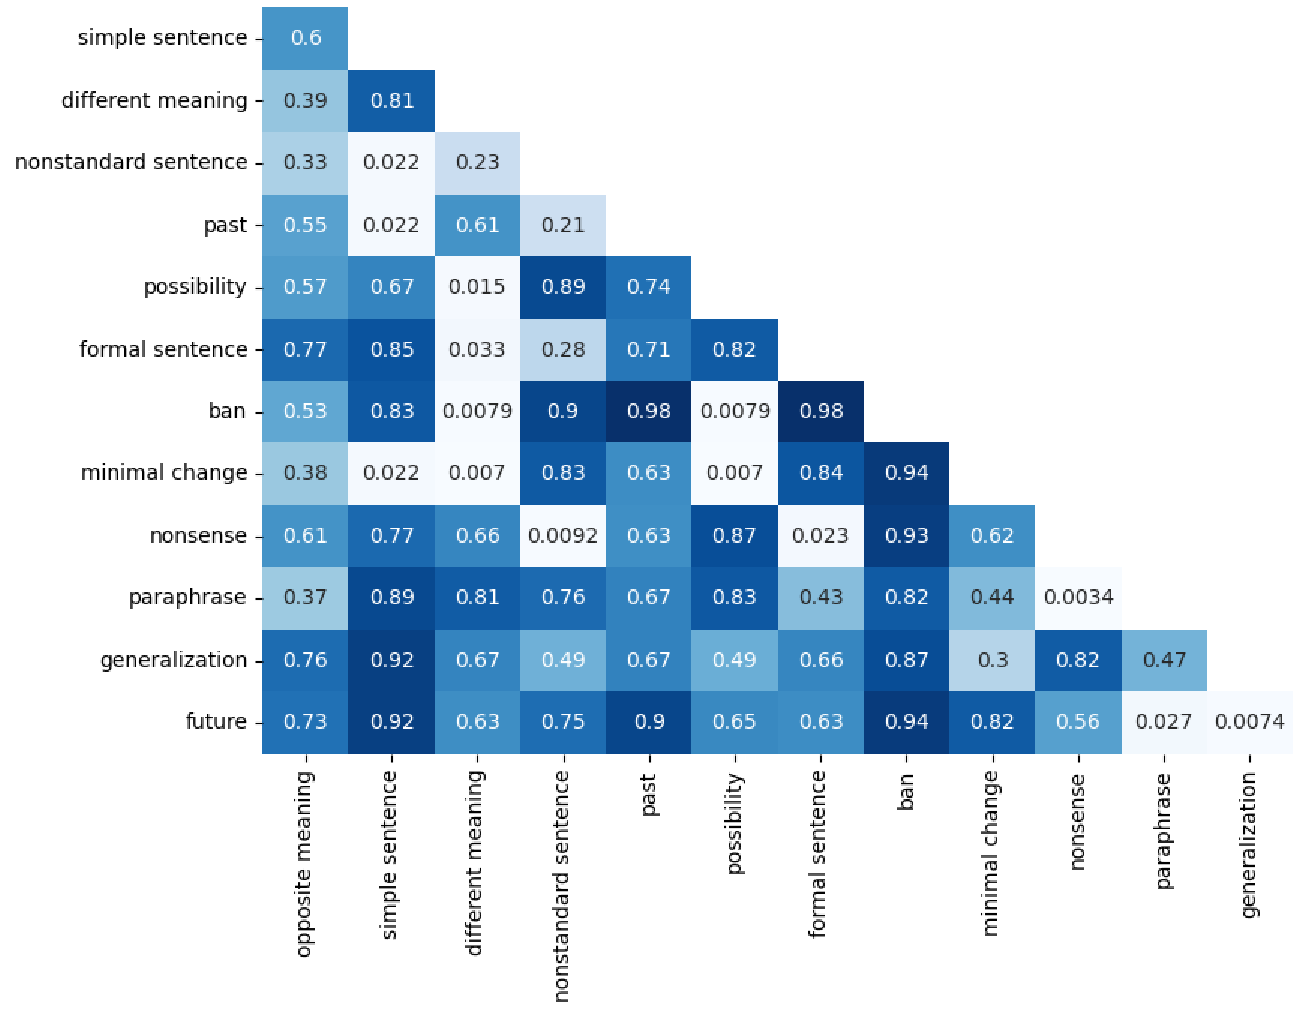
\includegraphics[scale=0.4]{GM.png}
    \caption{Accuracy of Measured Separability with Gaussian Mixture}
    \label{fig:GM}
\end{figure}





% \subsection{SBERT as a classifier}
% This section shows whether the sentence embeddings trained on our models can serve as a classifier and separate sentences in terms of labels.

% For each derivation sentence, we compute the distance from its seed. The resulting vector. It is assumed that a certain type of derivation from a seed shares some similarities. A good classifier is assumed to group the same derivation types. For example, (sentence vector - seed vector)sentences with future tense are supposed to group together.
% visualize the distance vecotors 

% reduced dimension PCA


% Sentence embeddings trained with SBERT can serve as classifier for some labels. For instance, the embeddings can separate 'future','past' and 'simple sentence' as in Figure X
% However, it does not work for the rest of groups: 

% \subsection{Degree of Transformation}

% Whether the degree of transformation can be characterized by SBERT sentence embeddings. 
% It shows the generalization group achieved most correlation.
% The more generalized sentences are further from seed sentence. While less generalized sentences (sentence meaning closer to seed sentences) has shorter distance to seed sentences


\bibliography{anthology}
\bibliographystyle{acl_natbib}


\end{document}
